\clearpage
\renewcommand{\thesection}{S.\arabic{section}}
\renewcommand{\thesubsection}{\thesection.\arabic{subsection}}
\renewcommand{\thefigure}{S.\arabic{figure}}
\renewcommand{\thetable}{S.\arabic{table}}

\makeatletter
\long\def\theequation{S\@arabic \c@equation}
\makeatother
\setcounter{page}{1}
\setcounter{figure}{0}
\setcounter{section}{0}
\setcounter{table}{0}

\onecolumn
\begin{bibunit}
\section{Supplementary Information}
\label{sec:supplementary}
\subsection{Dependencies of \gs}
\label{sec:dependencies}
We here list and discuss external packages that \gs depend on.
Except for the foremost dependency \citet{MATLAB2014}, these packages are freely available online for academic use.
No dependency is currently a hard dependency, meaning that except for specific functionality, most of \gs can be used without these packages.

\begin{itemize}
\item \href{https://git-scm.com/}{git} for easily keeping up to date with the GeneSPIDER toolbox.
\item \href{https://web.stanford.edu/~hastie/glmnet_matlab/}{Glmnet} \citep{Friedman2010} is used within wrapper functions, such as \texttt{Methods.Glmnet}, \texttt{Methods.Bolasso}.
\item \href{http://www.mathworks.com/matlabcentral/fileexchange/33381-jsonlab--a-toolbox-to-encode-decode-json-files-in-matlab-octave}{JSONlab} for exporting to storage format .json or .ubj.
\item \href{https://www.mathworks.com/matlabcentral/fileexchange/6268-xml4mat-v2-0}{xml4mat} is necessary for exporting data to the xml storage format.
\item \href{http://cvxr.com/cvx/}{CVX} for disciplined convex programming in some of our in-house inference methods.
\item \href{https://bitbucket.org/nordron/nordron-rni}{RInorm} \citep{Nordling2013phdthesis} for robust network inference using the algorithm by \href{http://www.nordron.com}{Nordron AB}.
\item \href{http://califano.c2b2.columbia.edu/ARACNe/}{ARACNe2} for the ARACNe wrapper. Configuration files needs to be set as per instructions for ARACNe default or per users specific use cases. The PATH to the ARACNe home directory needs to be set before MATLAB is started.
\end{itemize}

\subsection{Installation instructions}
\label{sec:install_instructions}

To fetch the \gs repository run the command:
\begin{verbatim}
git clone git@bitbucket.org:sonnhammergrni/genespider.git ~/src/genespider
\end{verbatim}
or download it from \url{https://bitbucket.org/sonnhammergrni/genespider} to \texttt{\textasciitilde{}/src/genespider}.
Change to the directory where you downloaded the repository by \texttt{cd \textasciitilde{}/src/genespider}.
Next, to fetch the complete \gs package run the following:
\begin{verbatim}
git submodule init
git submodule update
\end{verbatim}
\gs will be available after adding the path \texttt{\textasciitilde{}/src/genespider} to your MATLAB path with the command:
\begin{verbatim}
addpath('~/src/genespider')
\end{verbatim}

To develop and keep track of changes for each submodule separately, you need to check out the master branch from each submodule with the command \texttt{git checkout master}. Each toolbox is expecting to be treated as a MATLAB toolbox \ie that a \texttt{+} prepended on each directory and the parent directory is added to the MATLAB path.


\subsection{Notation used for steady-state data}
\label{sec:SSnotation}
Assuming that data is recorded during steady-state, the system (\ref{eq:linearsys}) simplifies to a linear mapping
\begin{equation}
  \mY = -\check{\mA}^{-1}(\mP - \mF) + \mE .
  \label{eq:Linearmap}
\end{equation}

\noindent
Here \(\mY \triangleq [\by_1,\ldots,\by_M]\) is the measured steady-state response matrix after applying the perturbations \(\mP \triangleq [\bp_1,\ldots,\bp_M]\) in \(M\) experiments and \(\check{\mA}\) is the interaction matrix.

An alternative representation that is commonly used in regression problems is obtained by taking the transpose of the variables and ``true'' network model. We obtain the matrix form of the standard linear data model used in errors-in-variables regression problems\index{errors-in-variables}\index{regression problem} by introducing the notation used for regressors \({\mPhi} \triangleq [{\bphi}_{1},\ldots,{\bphi}_{j},\ldots,{\bphi}_{\breve{N}}] = \mY^{T}\), regressands \({\mXi} \triangleq [{\bxi}_{1},\ldots,{\bxi}_{i},\ldots,{\bxi}_{\breve{N}}] = -\mP^{T}\), regressor errors \({\mUpsilon} \triangleq [{\bupsilon}_{1},\ldots,\bupsilon_{j},\ldots{\bupsilon}_{\breve{N}}]=\mE^{T}\), and regressand errors \({\mPi} \triangleq [{\bepsilon}_{1},\ldots,\bepsilon_{i},\ldots{\bepsilon}_{\breve{N}}]=-\mF^{T}\).
\begin{subequations}\label{eqn:MatrixEquationWithErrorsConvertedToRegressors}
  \begin{align}
    & \hspace{-2mm} {\mPhi}  = \check{\mPhi} + \mUpsilon, && \mXi = \check{\mXi} + \mPi   \\
    & \hspace{-2mm} \check{\mPhi} \check{\mA}^{T} = \check{\mXi} && \mPhi, \mXi \in \mathbb{R}^{\breve{M} \times \breve{N}} .
    \label{eqn:MatrixEquationWithErrorsConvertedToRegressorsSystem}
  \end{align}
\end{subequations}

\noindent


\subsection{Toolboxes}
\label{sec:toolboxes}
\subsubsection{Data structure toolbox}
\label{sec:datastruct_toolbox}
This toolbox provides the two main data type classes for networks and experimental data: \texttt{Network} and \texttt{Dataset}.
This division reflects the fact that one network is commonly used to generate many different \insilico datasets and that experimental data collected from an unknown network need to be stored without any network.
Table \ref{tab:datastruct} lists all classes and functions available within this toolbox.

Storing and loading data and networks is an important part of network inference work, and we have therefore opted to include multiple storage formats for the data types.
These include \matlab's native format \texttt{.mat} files, which make it easy to save and load data, \emph{Extensible Markup Language}
(XML), specifically \matlab markup language (mbml) \citep{Almeida2003} as \texttt{.xml} files, and \emph{JavaScript Object Notation} (JSON), which offers a wide range of possibilities for sharing and importing data in \matlab and other languages.
JSON comes with both the standard \texttt{.json} format, but also as a binary version, Universal Binary JSON \texttt{.ubj}.
% Both XML and JSON functionality is provided by external open source libraries (see section \ref{sec:dependencies}). \textcolor{red}{
Despite its name, the export2Cytoscape function also imports networks.%}
% \textcolor{red}{
Three normalisation methods are available for a dataset object,
standard normalization \(\hat{x}_{i} = \frac{x_{i}-\mu_{i}}{\sigma_{i}}\), min max range normalisation \(\hat{x}_{i} = \frac{x_{i} - \min(x_{i})}{\max(x_{i}) - \min(x_{i})}\), and unit length normalisation \(\hat{x}_{i} = \frac{x_{i}}{||x_{i}||}\). Here \(\hat{x}_{i}\) is the normalised variable or sample of \(x_{i}\). \(\mu\) is the mean of sample \(i\) and \(\sigma\) the standard deviation, \(||.||\) is the 2 norm and \(\min\) and \(\max\) are the minimum and maximum operators.
Noise estimates needs to be redone after normalisation to be used to estimate new data properties.%}


\begin{table}[htb]
\caption{\label{tab:datastruct}
Contents of the \texttt{datastruct} toolbox.}
\centering
\begin{tabular}{|l|p{10cm}|}
\hline
Class or function & Description\\
\hline
Dataset & Stores a data set consisting of a perturbation (\(\mP\)) and response (\(\mY\)) matrix\\
Network & Stores a network matrix (\(\mA\))\\
\hline
RSS & Calculation of the residual sum of squares for responses and perturbations\\
cutSym & Removes links in a symmetric matrix with a probability to be in or out degree\\
expectedSNRv & Calculation of the expected \(\SNR_{\phi\, \normall}\)\\
export2Cytoscape & Exports a network to a tsv file that can be loaded in Cytoscape, as well as imports network files\\
optimalRandomP & Generates perturbations that counteract signal attenuation based on SVD of \(\mY\)\\
randomNet & Creates a random network with \(N\) nodes and specific sparseness with no self loops\\
scalefree & Create a scale-free network with \(N\) nodes and specific sparseness\\
smallworld & Generate a small-world network\\
stabalize & Weights a static network structure\\
simts & Simple simulation of a time-series response of the linear ODE model\\
weightP & Adjusts elements of \(\mP\) to bring the singular values of \(\mY\) close to one\\
\hline
\end{tabular}
\end{table}


\paragraph{The Network class}
\label{sec:network_class}
is a container for networks, in this case a linear model, represented by a matrix \(\boldsymbol{A}\).
All methods are listed in Table \ref{tab:network_class}.
Note that some native \matlab functionality is provided for this data type, such as \texttt{svd}, \texttt{logical}, \texttt{sign}, and \texttt{size} operations, and that also a method \texttt{fetch} for getting networks from the online repository at \url{https://bitbucket.org/sonnhammergrni/gs-networks} is provided.
The Network class is capable of handling sparse matrices.

\begin{table}[htb]
\caption{\label{tab:network_class}
Methods in the \texttt{Network} class.}
\centering
\begin{tabular}{|l|p{10cm}|}
\hline
Method & Description\\
\hline
fetch & Get GeneSPIDER networks from the online repository\\
load & Loads a dataset/network back in to a \texttt{datastruct}\\
save & Saves a \texttt{datastruct} object to file, as a .mat, .json, .ubj, or .xml file.\\
populate & Populates the \texttt{Network} object with matching fields of an input struct\\
nnz & Returns the number of non zero entries in the network\\
size & Returns the size of the network\\
sign & Returns the signed structure of the network\\
logical & Returns the logical structure of the network\\
svd & Returns the singular values of \(A\). To get the singular vectors use \texttt{svd(net.A)}\\
view & Makes a rough graphical network plot using biograph\\
\hline
\end{tabular}
\end{table}


\paragraph{The Dataset class}
\label{sec:dataset_class}
is a container for data sets, i.e. perturbation and response data from experiments.
It provides a number of functionalities related to data handling, listed in Table \ref{tab:dataset}.

\begin{table}[htb]
\caption{\label{tab:dataset}
Methods in the \texttt{Dataset} class.}
\centering
\begin{tabular}{|l|p{10cm}|}
\hline
Method & Description\\
\hline
bootstrap & Bootstraps a new data set from the old data set\\
eta & Calculates the sample-wise linear dependence \(\eta\) of \(\mY\) and \(\mP\)\\
gaussian & Generates Gaussian noise matrices \(\mE\) and \(\mF\) with variance \(\lambda\)\\
include & Returns samples that can be include in LOOCO based on the \(\eta\) limit\\
populate & Populates the \texttt{Dataset} object with matching fields of an input struct\\
response & Returns the noisy steady-state response of the network\\
save & Saves a \texttt{datastruct} object to file, as a .mat, .json, .ubj, or .xml file\\
load & Loads a dataset file back in to a \texttt{datastruct}\\
fetch & Loads a dataset from the on-line repository via URL or name\\
scaleSNR & Scales the noise variance to achieve the desired SNR\\
std & Returns the standard deviation of all data points\\
true\_response & Returns the noise-free steady-state response of the network\\
w\_eta & Calculates SVD based sample-wise linear dependence \(\eta\) of \(\mY\) and \(\mP\)\\
without & Creates a \texttt{Dataset} without sample \(i\)\\
\textcolor{red}{std\_normalize }& \textcolor{red}{Creates a \texttt{Dataset} with standard normalised expression values}\\
\textcolor{red}{range\_scaling} & \textcolor{red}{Creates a \texttt{Dataset} with \texttt{min max} scaling}\\
\textcolor{red}{unit\_length\_scaling} & \textcolor{red}{Creates a \texttt{Dataset} with unit length  scaling}\\
\hline
\end{tabular}
\end{table}

\subsubsection{Analysis toolbox}
\label{sec:analysis_toolbox}
Provides fundamental, as well as complex functions for analysing data and models.
These are listed in Table \ref{tab:analyse}.

\begin{table}[htb]
\caption{\label{tab:analyse}
Contents of the \texttt{analyse} toolbox.}
\centering
\begin{tabular}{|l|p{10cm}|}
\hline
Class or function & Description\\
\hline
Model & Calculates properties related to the supplied \texttt{Network}\\
CompareModels & Calculates similarity measures of weighted network adjacency matrices\\
Data & Calculates data properties of the supplied \texttt{Dataset}\\
\hline
\end{tabular}
\end{table}


\paragraph{The Model class}
\label{sec:model_class}
is aimed at analysing models/networks.
It provide measures to quantify the properties of the network. The methods are listed in Table \ref{tab:model}.
Specification of how to treat links (directed or undirected) in measures that depend on the link type is supported.

\begin{table}[htb]
\caption{\label{tab:model}
Methods of \texttt{Model} class.}
\centering
\begin{tabular}{|l|p{10cm}|}
\hline
Method & Description\\
\hline
alpha & Returns the significance level (default 0.01)\\
analyse\_model & Batch calculation of almost all the measures below (used internally)\\
calc\_proximity\_ratio & Calculates the proximity ratio or "small-worldness" tendency of the network\\
clustering\_coefficient & Calculates the clustering coefficient\\
cond & Calculates the condition number of the network \(\mA\)\\
degree\_distribution & Calculates the degree distribution\\
graphconncomp & Finds the strongly connected components of the graph\\
identifier & Returns the name of the network\\
median\_path\_length & Calculates the mean and median path length\\
time\_constant & Calculates the smallest time constant of the system based on \(\mA\)\\
tol & Sets a tolerance value for computations if it is needed\\
type & Returns the type of the graph, i.e. 'directed' or 'undirected'\\
\hline
\end{tabular}
\end{table}

\paragraph{The Data class}
\label{sec:data_class}
is included for analysis and quantification of data properties. The methods are listed in Table \ref{tab:data}.
All measures are calculated and reported at an adjustable significance level, with default value \(\alpha = 0.01\).

\begin{table}[htb]
\caption{\label{tab:data}
Methods of \texttt{Data} class.}
\centering
\begin{tabular}{|l|p{10cm}|}
\hline
Method & Description\\
\hline
alpha & Returns the significance level (default 0.01)\\
analyse\_data & Batch calculation of almost all the measures below\\
calc\_SNR\_Phi\_gauss & Calculates the SNR as defined in equation (\ref{eq:SNR-Phi-N})\\
calc\_SNR\_Phi\_true & Calculates the SNR as defined in equation (\ref{eq:SNR-Phi-true})\\
calc\_SNR\_phi\_gauss & Calculates the SNR as defined in equation (\ref{eq:SNR-phi-min})\\
calc\_SNR\_phi\_true & Calculates the SNR as defined in equation (\ref{eq:SNR-phi})\\
irrepresentability & Calculates the strong irrepresentable condition\\
tol & Sets a tolerance value for computations if it is needed\\
\hline
\end{tabular}
\end{table}

\paragraph{The CompareModels class}
\label{sec:compare-models}
can be used to compare networks to each other.
A number of different measures are computed and reported, see Table \ref{tab:sys-measures} -  \ref{tab:dir-graph-measures}.
If the supplied golden standard network is not square, then \texttt{CompareModels} will calculate the similarity of off-diagonal elements, by assuming that the diagonal has been removed and truncated along the second dimension.
Table \ref{tab:compare_functionality} is a reference for the methods that can be used with the CompareModels class. They add additional measures AUROC and AUPR (using "trapz" matlab function \cite{MATLAB2014}) and methods to save, store and transfer results to other environments.

\begin{table}[htb]
\caption{\label{tab:sys-measures}
System measures}
\centering
\begin{tabular}{|l|p{8cm}|}
\hline
Name & Description\\
\hline
abs2norm & Absolute induced 2-norm\\
rel2norm & Relative induced 2-norm\\
maee & Max absolute element error\\
mree & Max relative element error\\
mase & Max absolute singular value error\\
mrse & Max relative singular value error\\
masde & Max absolute singular direction error\\
mrsde & Max relative singular direction error\\
maeve & Max absolute eigen value error\\
mreve & Max relative eigen value error\\
maede & Max absolute eigen direction error\\
mrede & Max relative eigen direction error\\
afronorm & Absolute Frobenius norm equivalent to 2-norm of A vectorised\\
rfronorm & Relative Frobenius norm\\
al1norm & l1-norm of zero elements\\
rl1norm & Relative l1-norm of zero elements\\
n0larger & \# zero elements larger than smallest nonzero element of A\\
r0larger & \# zero elements larger than smallest nonzero element of A/\# zero elements in A\\
\hline
\end{tabular}
\end{table}


\begin{table}[htb]
\caption{\label{tab:signed-topo-measures}
Signed topology measures}
\centering
\begin{tabular}{|l|p{8cm}|}
\hline
Name & Description\\
\hline
ncs & \# Correct signs\\
sst & Similarity of signed topology\\
sst0 & Similarity of signed topology of non-zero elements of A\\
\hline
\end{tabular}
\end{table}


\begin{table}[htb]
\caption{\label{tab:corr-measures}
Correlation measures}
\centering
\begin{tabular}{|l|p{8cm}|}
\hline
Name & Description\\
\hline
plc & Pearson's linear correlation coefficient\\
\hline
\end{tabular}
\end{table}

\begin{table}[htb]
\caption{\label{tab:graph-measures}
Graph measures}
\centering
\begin{tabular}{|l|p{8cm}|}
\hline
Name & Description\\
\hline
nlinks & \# Links in estimated network\\
TP & \# True Positives\\
TN & \# True Negatives\\
FP & \# False Positives\\
FN & \# False Negatives\\
sen & Sensitivity TP/(TP+FN)\\
spe & Specificity TN/(TN+FP)\\
comspe & Complementary specificity 1-Specificity\\
pre & Precision TP/(TP+FP)\\
TPTN & Number of links that is present and absent in both networks (TP+TN)\\
structsim & Structural similarity (TP+TN)/\#Nodes\^{}2\\
MCC & Matthews correlation coefficient\\
\hline
\end{tabular}
\end{table}


\begin{table}[htb]
\caption{\label{tab:dir-graph-measures}
Directed graph measures}
\centering
\begin{tabular}{|l|p{8cm}|}
\hline
Name & Description\\
\hline
TR & True Regulation\\
TZ & True Zero\\
FI & False Interaction\\
FR & False Regulation\\
FZ & False Zero\\
dirsen & Directed sensitivity\\
dirspe & Directed specificity\\
dirprec & Directed precision\\
SMCC & Signed Matthews correlation coefficient\\
\hline
\end{tabular}
\end{table}


\begin{table}[htb]
\caption{\label{tab:compare_functionality}
Methods in the CompareModels class}
\centering
\begin{tabular}{|l|p{8cm}|}
\hline
Name & Description\\
\hline
AUROC & Calculate area under ROC curve\\
ROC & Plot ROC curve\\
AUPR & Calculate area under PR curve\\
PR & Plot PR curve\\
save & save the comparison in specified format. Most formats that MATLAB datasets can be saved in are supported as well as json format if the jsonlab dependency is met\\
\hline
\end{tabular}
\end{table}


\subsubsection{Methods toolbox}
\label{sec:methods_toolbox}
Provides mainly wrapper functionality for inference methods.
These wrapper functions are written in relation to a specific inference method and accepts as
input a standard set of variables: a \texttt{Dataset} object,
an optional \texttt{Network} object, and a regularisation penalty value array.
These are handled internally by the wrapper, which output an inferred network or array of inferred networks.
The common interface for each function looks as follows:
\begin{verbatim}
zetavec = logspace(-6,0,10);
estA = Methods.method_name(Data,zetavec)
\end{verbatim}
Here \texttt{Data} is the generated data object, and \texttt{zetavec} is a vector of regularisation parameters required by the method.
The inferred networks are returned in \texttt{estA}.
The available methods are listed in \ref{tab:gs-methods}.
An alternative way of running the methods presented in this paper is also provided, where the regularization parameter range can be estimated by the method wrapper itself
\begin{verbatim}
[estA,zetavec,zetaRange] = Methods.method_name(Data,'full')
\end{verbatim}
Calling the wrapper in this way will return a scaled zetavec $\in [0,1]$ where if possible all regularisation steps are included, and the scaling factors in zetaRange that can be used to rescale the zetavec to its actual range.

\begin{table}[htb]
\caption{\label{tab:gs-methods}
Method wrappers in \gs. Each method can be called with a simple unified structure: \texttt{Methods.<function>(<data>,<parameters>)}.}
\centering
\begin{tabular}{|l|l|l|}
\hline
function & reference & note\\
\hline
Glmnet & \citet{Friedman2010} & \lasso/elastic net/ridge regression\\
NIR & \citet{DiBernardo2004} & Exhaustive subset regression\\
Bolasso & \citet{Bach2008} & Bootstrap utilising Glmnet\\
ccd & \citet{abenius2010report} & Cyclic coordinate descent\\
Glasso & \citet{Friedman2008} & Graphical lasso\\
LARS & \citet{Sjostrand2005} & Least angular regression\\
RNI & \citet{Nordling2013phdthesis} & Robust network inference\\
julius & \citet{Julius2009} & \lasso based convex programming\\
lsco & \citet{Tjarnberg2013} & Least squares cut-off\\
fcls & \citet{Tjarnberg2013} & Fast constrained least squares\\
ARACNe & \citet{margolin2006ARACNe} & Algorithm for the Reconstruction of Accurate Cellular Networks\\
\hline
\end{tabular}
\end{table}



Our in-house implementations of algorithms include Least Squares with Cut-Off (LSCO) and Total Least Squares with Cut-Off (TLSCO),
\begin{equation}\label{eqn:tLSCO}
  \hat{a}_{ij} \triangleq \left\{
    \begin{array}{ll}  a_{ij}^{*ls} & \textrm{if}\; a_{ij}^{*ls} \geq \tilde{\zeta}\\
      0 & \textrm{otherwise}
    \end{array} \right.
%\; \textrm{with} \; \mA_{*ls} = -\bP\bY^{\dagger}.
\end{equation}

\noindent
where \(\mA_{*ls}\) is either the total or ordinary least squares estimate.
We have also implemented a bootstrap approach for both the LSCO and the TLSCO algorithms.

An optimised implementation of the structurally constrained least squares (CLS) is also provided, which minimises the bias introduced by the regularisation term of \eg \lasso, by solving
\begin{subequations}\label{eqn:CLS}
\begin{align}\label{eqn:CLSObj}
  \hat{\mA} = \arg \min_{\mA} & \sum \diag(\mDelta^T\mR \mDelta) \\
  \text{s.t.}\; & \mDelta = \mA \mY + \mP, \label{eqn:CLSPredErr} \\
  & \mR = \left( \hat{\mA}_{\textrm{init}} \Cov[\by] \hat{\mA}_{\textrm{init}}^{T} + \Cov[\bp]\right)^{-1}, \label{eqn:CLSR} \\
  & \sign{\mA} = \sign{\hat{\mA}_{\textrm{reg}}}. \label{eqn:CLSStructure}
\end{align}
\end{subequations}

\noindent
Here \(\hat{\mA}_{\textrm{reg}}\) denotes the network estimate given by the regularisation method, \eg \lasso, \(\Cov[\by]\) the covariance matrix of the response in an experiment or an estimate of it, \(\Cov[\bp]\) the covariance matrix of the perturbation in an experiment or an estimate of it, and \(\sign\) the signum function.
The structure of the network is forced to be identical to the estimate given by the regularisation method by the last constraint in the optimisation problem.
Ideally, the network estimate \(\hat{\mA}\) should be used instead of \(\hat{\mA}_{\textrm{init}}\), but then the problem is not convex.
In practice one should therefore solve this problem iteratively, starting with \(\hat{\mA}_{\textrm{init}} = \hat{\mA}_{\textrm{reg}}\) in the first iteration and then \(\hat{\mA}_{\textrm{init}}\) equal to the estimate from the last iteration \(\hat{\mA}\) until the estimate has converged with desired precision.
This method is based on the method presented in \citep{Julius2009}, where the covariance is assumed to be identical in all experiments.


\subsubsection{gsUtilities toolbox}
\label{sec:gsUtilities}
Provides miscellaneous helper functions listed in \ref{tab:tool}.

\begin{table}[htb]
\caption{\label{tab:tool}
Contents of the \texttt{gsUtilities} toolbox.}
\centering
\begin{tabular}{|l|p{10cm}|}
\hline
Class or function & Description\\
\hline
export2gnuplot & Export of vectors and variables to a gnuplot friendly tsv format\\
optionParser & Parses input options into a struct\\
rmdiag & Removes diagonal elements and shifts the upper triangular elements -1 along the second dimension\\
sic & Calculates the strong irrepresentable condition\\
standardize & Standardises and normalises a given matrix\\
\hline
\end{tabular}
\end{table}




\subsection{Definitions of data properties}
\label{sec:def-data-prop}
We here define several data properties provided by \gs.

\subsubsection{Signal to Noise Ratio}
\label{sec:SNR}
The signal to noise ratio (SNR) can be defined in many different ways and we have implemented several of them in order to evaluate them.
In general the SNR should be the ratio of the signal and uncertainty of the gene of interest \citep{Nordling2013phdthesis}
\begin{equation}
  \text{SNR}({\bphi}_j) \triangleq \frac{\norm{\bphi_j}}{r_{\mathcal{U}_{\bphi_j}}}\label{eq:SNR-phi}\\
\end{equation}

\noindent
where the radius of uncertainty set \(\mathcal{U}_{\bphi_{j}}\) is
\begin{equation}
  r_{\mathcal{U}_{\bphi_{j}}} \triangleq \underset{\tilde{\bphi}_j \in \mathcal{U}^{\alpha}_{\bphi_j}}{\sup} \norm{\tilde{{\bphi}_j}-{\bphi_j}}
\end{equation}

\noindent
From (\ref{eq:Linearmap}) we can derive an expression of the SNR considering only output noise
\begin{equation}
  \SNR_{\mPhi\, true} \triangleq \frac{\underline\sigma(\mY)}{\overline\sigma(\mE)} = \frac{\underline\sigma(\mPhi)}{\overline\sigma(\mUpsilon)}. \label{eq:SNR-Phi-true}
\end{equation}

\noindent
Here \(\overline{\sigma}\) represent the largest singular value and \(\underline{\sigma}\) represent the smallest non-zero singular value.
Note that the noise matrix \(\mE\) is only available for \insilico data.
We therefore also define a corresponding measure based on assumption of the noise being normally distributed with variance \(\lambda\)
\begin{align}%{lr}
  \SNR_{\mPhi\, \normall} \triangleq & \frac{\underline{\sigma}(\bPhi)}{\sqrt{\chi^{-2}(\alpha,NM)\lambda}} \label{eq:SNR-Phi-N} .
% \label{eq:SNR-N-def}
\end{align}

\noindent
Here \(\normall\) indicates that the noise is assumed to follow a normal distribution with mean \(\mu\), variance \(\lambda_{(i)}\) and \(\chi^{-2}(\alpha,NM)\) is the inverse chi-square distribution with \(NM\) degrees of freedom at significance level \(\alpha\).
We also define SNRs for individual genes:
\begin{subequations} \label{eq:SNR-def}
    \begin{align}%{lr}
      \SNR_{\phi\, \normall} \triangleq & \argmin_i\frac{\norm{\bphi_i}}{\sqrt{\chi^{-2}(\alpha,N)\lambda_i}}\\
      \SNR_{\phi\,true} \triangleq & \argmin_i \frac{\norm{\bphi_i}}{\norm{\bupsilon_i}} \label{eq:SNR-phi-min}\\
      \langle\SNR\rangle_{\phi\, \normall} \triangleq & \mean_i\frac{\norm{\bphi_i}}{\sqrt{\chi^{-2}(\alpha,N)\lambda_i}}\\
      \langle\SNR\rangle_{\phi\, true} \triangleq & \mean_i \frac{\norm{\bphi_i}}{\norm{\bupsilon_i}}.
    \end{align}
\end{subequations}

\noindent



\subsubsection{Sample-wise linear dependence}
\label{sec:linear_dependence}

An experiment can only be predicted through a model based upon data reflective of the underlying system properties, \eg a closely related experiment.
This implies that it is essential to filter the experiments before using any leave-one-out cross-validation or cross-optimisation strategy \citep{Tjarnberg2013}.
If an experiment is linearly dependent on other experiments then the latter contain information about the former, and thus one should estimate the linear independence of the samples, \(\eta_{\by_k}\) and \(\eta_{\bp_k}\),
\begin{align}
  \eta_{\by_k} \triangleq ||\bY^T_{t\neq k} \by_k||_1  &&  \eta_{\bp_k} \triangleq ||\bP^T_{t\neq k} \bp_k||_1 .
  \label{eq:eta}
\end{align}

\noindent
Only samples fulfilling
\begin{align}
  \mathcal{V} & \triangleq \big\{k| \eta_{\by_k} \geq \sigma_N(\mY) \; \textrm{and}\; \eta_{\bp_k} \geq \sigma_N(\mP) \big\}
  \label{eq:etaexperiments}
\end{align}

\noindent
should be included.

\subsection{Generating example data as used in results section}
\label{sec:example}
\gs provides four \matlab toolboxes: \texttt{datastruct}, \texttt{analyse},
\texttt{Methods}, and \texttt{gsUtilities}.
Each toolbox is aimed at a specific function and their usage is exemplified here.
The data used in the examples below can be downloaded from the online repository at \url{https://bitbucket.org/sonnhammergrni/gs-networks}. The network is \href{https://bitbucket.org/sonnhammergrni/gs-networks/raw/ec384db2750b5ef229d1c613e3dd04a5e3b634e2/random/N10/Nordling-D20100302-random-N10-L25-ID1446937.json}{Nordling-D20100302-random-N10-L25-ID1446937} and dataset is \href{https://bitbucket.org/sonnhammergrni/gs-datasets/raw/a9d9b00aaa5fa6f4059ba03fd0cb5ec8eb80f3f0/N10/Nordling-ID1446937-D20150825-E15-SNR3291-IDY15968.json}{Nordling-ID1446937-D20150825-E15-SNR3291-IDY15968}.
Note that if the code below is used to generate a new network and dataset, then they will differ from the presented ones due to the use of random number generators to create the network and noise matrices.

\subsubsection{Network generation}
\label{sec:Network_generation_example}
We start by generating a stable random network with \(10\) nodes and sparsity \(0.25\).
The following code snippet demonstrate how to create a
\texttt{datastruct.Network} object with the above specifications.
\begin{verbatim}
N = 10; S=0.25;
A = datastruct.randomNet(N,S)-eye(N);
A = datastruct.stabalize(A,'iaa','high');
Net = datastruct.Network(A,'random');
setname(Net,struct('creator','Nordling'));
Net.description = ['This is a sparse network with 10 nodes,'...
    '10 negative self-loops and 15 randomly chosen'...
    'links generated by Nordling 2010-03-02.'...
    'The coefficients are chosen such that they form one'...
    'strong component and a stable dynamical system with'...
    'time constants in the range 0.089 to 12 and an'...
    'interampatteness level of 145 that is in-between'...
    'the estimated level of an E. coli (Gardner et al. 2003 Science)'...
    'and Yeast (Lorenz et al. 2009 PNAS) gene regulatory network.'...
    'The coefficients of the network have not been tuned to explain'...
    'any of the data sets in the mentioned articles.'];
\end{verbatim}
\texttt{datastruct.stabalize} takes the random network and the desired IAA as input parameters and stabilises the network by making the real part of all eigenvalues negative while adjusting the IAA level.
The \texttt{setname} method is used to specify the fields of the \texttt{Network} object.
The name is automatically generated based on the network properties to ensure that each one is unique.

The displayed output of the \texttt{Network} object is in this case:
\begin{verbatim}
Net =

  10x10 Network array with properties:

              network: 'Nordling-D20100302-random-N10-L25-ID1446937'
                    A: [10x10 double]
                    G: [10x10 double]
                names: {'G1' 'G2' 'G3' 'G4' 'G5' 'G6' 'G7' 'G8' 'G9' 'G10'}
                 desc: 'This is a sparse network with 10 nodes, 10 negative
                        self-loop and 15 randomly chosen links generated by
                        Nordling 2010-03-02. The coefficients are chosen such
                        that they forms one strong component and a stable
                        dynamical system with time constants in the range 0.089
                        to 12 and an interampatteness level of 145 that is in
                        between the estimated level of an
                        E. coli (Gardner et al. 2003 Science) and
                        Yeast (Lorenz et al. 2009 PNAS) gene regulatory network.
                        The coefficients of the network have not been tuned to
                        explain any of the data sets in the mentioned articles.'
\end{verbatim}
The displayed output shows the non-hidden properties of the \texttt{Network} object.
\texttt{network} is the name of the object, which contains the name of the creator \texttt{Nordling}, the date of creation \texttt{D}, the type of network \texttt{random}, the number of nodes, and the number of edges \texttt{L}.
\texttt{A} is the network matrix. \texttt{G} is the static gain matrix (inverse of \texttt{A}),
which is precomputed to save time when used in an inference algorithm.
\texttt{names} contains the name assigned to each node, which are generated automatically if they are not specified.
\texttt{desc} is a description of the network.
The Network class can handle sparse matrices.

For the example in this article, we generated 10 networks of each size, \(N\in \{10,50,100\}\), each of the four classes, random, small-world, scale-free and small-world-scale-free, and each of two IAA levels, \(\kappa \in \{low,high\}\), giving a total of 240 networks.
The IAA degree of each network is shown in Figure \ref{fig:iaa}.
The degree distributions for each network topology class and size are shown in Figure \ref{fig:out-degree}.
\begin{figure*}
[!htbp]
\centering
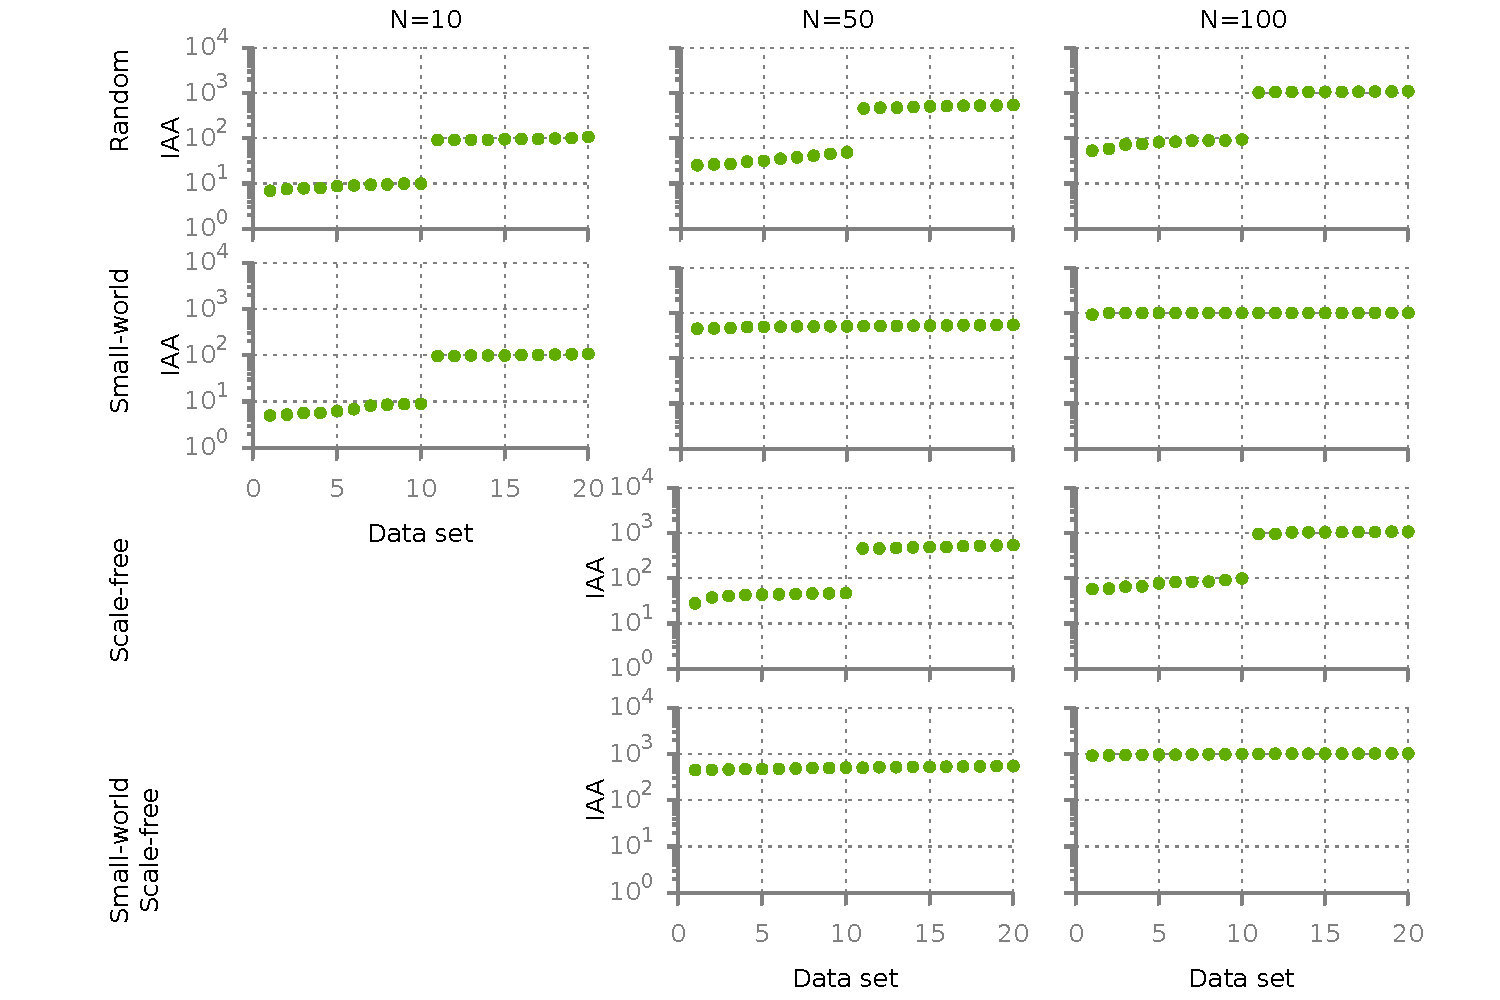
\includegraphics[width=.7\linewidth]{img/iaa_networks}
\captionsetup{width=.7\textwidth}
\caption{Interampatteness degrees for the networks in the benchmark suite. Each point represents a network, with its IAA degree on the y-axis and its number in order of increasing IAA on the x-axis. The numbering is the same as in Figure \ref{fig:k-data}.}
\label{fig:iaa}
\end{figure*}

\begin{figure*}
[!htbp]
\centering
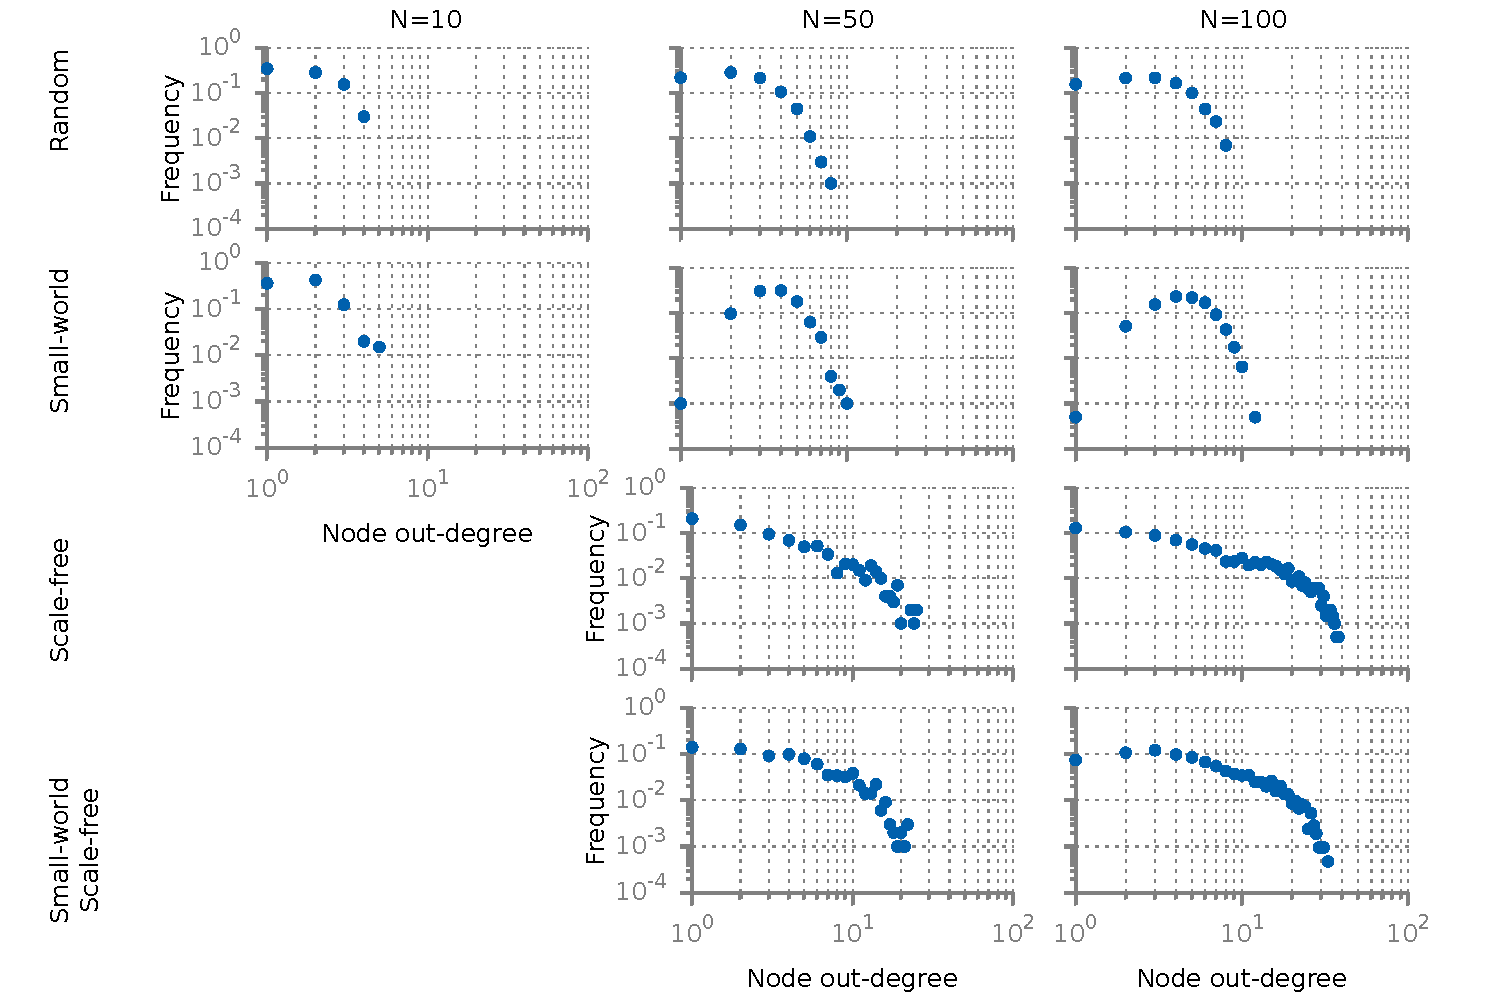
\includegraphics[width=.7\linewidth]{img/degree_distributions}
\captionsetup{width=.7\textwidth}
\caption{Out-degree distributions for the networks in the benchmark suite. Each distribution is based on 20 individual networks. The y-axis shows the degree frequency, and the x-axis shows the degree.}
\label{fig:out-degree}
\end{figure*}

\subsubsection{Data generation}
\label{sec:data-generation-example}
We now use the generated network to simulate perturbation experiments to obtain an expression dataset.
The following code snippet simulates \(N\) single gene perturbation experiments where each gene is perturbed one by one followed by \(N/2\) experiments in which genes are perturbed randomly.
\begin{verbatim}
SNR = 7;
P = double([eye(N),full(logical(sprandn(N,round(N/2),0.2)))]);
Y = Net.G*P;
s = svd(Y);
stdE = s(N)/(SNR*sqrt(chi2inv(1-analyse.Data.alpha,prod(size(P)))));
E = stdE*randn(size(P));
F = zeros(size(P));
\end{verbatim}
We have created a perturbation matrix \texttt{P} and a corresponding response matrix \texttt{Y}.
The standard deviation has been selected such that the SNR became 7 when it was used to generate the noise matrix \texttt{E}.
We didn't use the input noise matrix \texttt{F} here, but it needs to be specified, so it was set to zero.
With this information, we build a data struct, which we later use to populate the \texttt{Dataset} object.
\begin{verbatim}
D(1).network = Net.network;
D(1).E = E;
D(1).F = F;
D(1).Y = Y+D.E;
D(1).P = P;
D(1).lambda = [stdE^2,0];
D(1).cvY = D.lambda(1)*eye(N);
D(1).cvP = zeros(N);
D(1).sdY = stdE*ones(size(D.P));
D(1).sdP = zeros(size(D.P));
\end{verbatim}

The two easiest ways to populate the \texttt{Dataset} object with generated data is to either initialise it with the data and/or network or to use the function \texttt{populate}.
To initialise the \texttt{datastruct.Dataset} object with data we do the following:
\begin{verbatim}
Data = datastruct.Dataset(D,Net);
setname(Data,struct('creator','Nordling'));
data.description = ['This data set contains 15 simulated experiments with additive'...
    'white Gaussian noise with variance 0.00028 added to the response'...
    'in order to make the SNR 7 and the data partly informative for'...
    'network inference. The singular values of the response matrix'...
    'are in the range 0.77 to 1.2.'];
\end{verbatim}

The displayed output of the \texttt{Dataset} object is in this case:
\begin{verbatim}
Data =

Dataset with properties:

      dataset: 'Nordling-ID1446937-D20150825-E15-SNR3291-IDY15968'
      network: 'Nordling-D20100302-random-N10-L25-ID1446937'
            P: [10x15 double]
            F: [10x15 double]
          cvP: [10x10 double]
          sdP: [10x15 double]
            Y: [10x15 double]
            E: [10x15 double]
          cvY: [10x10 double]
          sdY: [10x15 double]
       lambda: [0.00028399 0]
        SNR_L: 3.2912
        names: {'G01'  'G02'  'G03'  'G04'  'G05'  'G06'  'G07'  'G08'  'G09'  'G10'}
  description: 'This data set contains 15 simulated experiments with additive
               white Gaussian noise with variance 0.00028 added to the response
               in order to make the SNR 7 and the data partly informative for
               network inference. The singular values of the response matrix
               are in the range 0.77 to 1.2.'
\end{verbatim}
\noindent
It is important to be able to connect a dataset to a specific network if the data was generated \insilico, hence the network name
is reported in the \texttt{Data} object.

\subsubsection{Analysis}
\label{sec:analysis_toolbox}
The \texttt{analysis} toolbox provides tools to analyse data, networks, and benchmark results.

First we demonstrate how to load the correct network and dataset from the online repository:
\begin{verbatim}
v = version('-release');
if str2num(v(1:end-1)) >= 2015
    disp('Fetching example data online')
    Net = datastruct.Network.fetch('Nordling-D20100302-random-N10-L25-ID1446937.json')
    Data = datastruct.Dataset.fetch('Nordling-ID1446937-D20150825-E15-SNR3291-IDY15968.json')
else
    disp('Older versions of MATLAB does not support fetching datasets online.')
end
\end{verbatim}


\paragraph{Network analysis:}
\label{sec:network_analysis_example}
To analyse the network we input it to the \texttt{analyse.Model} module:
\begin{verbatim}
net_prop = analyse.Model(Net);
disp(net_prop)
\end{verbatim}
It produces the output:
\begin{verbatim}
net_prop =

  Model with properties:

              network: 'Nordling-D20100302-random-N10-L25-ID1446937'
     interampatteness: 144.6937
    NetworkComponents: 1
        AvgPathLength: 2.8778
                 tauG: 0.085032
                   CC: 0.1
                   DD: 1.5
\end{verbatim}

Six measures are calculated.
The interampatteness degree, \texttt{interampatteness}, is the number reported by
\texttt{cond(A)} in \matlab.  \texttt{NetworkComponents} is the number of
strongly connected components, as reported by the \matlab function
\texttt{graphconncomp}.  \texttt{AvgPathLength} is the average path length of
the graph of the network in question, as reported by
\texttt{graphallshortestpaths} in \matlab.  \texttt{tauG} is the time constant
of the system.  \texttt{CC} is the average Clustering coefficient, which
can be interpreted as the neighbourhood sparsity of each node in
the network, not considering the node itself. \texttt{DD} is the
average degree distribution of the model.
The property \texttt{analyse.Model.type} can be set to \texttt{directed} (default) or \texttt{undirected} depending on the network and the properties one wishes to calculate.
This is a persistent property, so the value will remain the default one until it is changed.

Individual properties can also be calculated, \eg
all clustering coefficients can be calculated by
\begin{verbatim}
disp(['Clustering coefficients of the network ',Net.network])
CCs = analyse.Model.clustering_coefficient(Net)
\end{verbatim}

\paragraph{Data analysis:}
\label{sec:data_analysis_example}
To analyse the data we input the \texttt{Dataset} object to the \texttt{analyse.Data} module:
\begin{verbatim}
data_prop = analyse.Data(Data);
disp(data_prop)
\end{verbatim}
It will result in the following output:
\begin{verbatim}
data_prop =

Data with properties:

        dataset: 'Nordling-ID1446937-D20150825-E15-SNR3291-IDY15968'
   SNR_Phi_true: 7
  SNR_Phi_gauss: 3.2912
   SNR_phi_true: 10.991
  SNR_phi_gauss: 10.341
\end{verbatim}
The SNRs reported here correspond the definitions in equations
(\ref{eq:SNR-Phi-N}) - (\ref{eq:SNR-phi-min}) by default.
However, the SNR is calculated for all \(i\) with the following two functions:
\begin{verbatim}
disp('SNR estimate based on actual noise matrix E for each variable')
SNRe = analyse.Data.calc_SNR_phi_true(Data);
disp(SNRe)
\end{verbatim}
\begin{verbatim}
disp('SNR estimate based on variance estimate each variable')
SNRl = analyse.Data.calc_SNR_phi_gauss(Data);
disp(SNRl)
\end{verbatim}

\paragraph{Performance evaluation:}
\label{sec:performance_eval}
To analyse the performance of an inference method we first need to generate an output.
This is accomplished easily thanks to the wrappers.
Each method has an associated wrapper that parses the data of the method itself.
To run the Glmnet \lasso implementation we execute:

\begin{verbatim}
[estA,zetavec,zetaRange] = Methods.Glmnet(Data,'full');
\end{verbatim}
The variable \texttt{zetavec} is the returned regularisation parameters that was used within the algorithm. The option "full" will instruct the method to try to generate the complete regularization path from full to empty network with the $\zeta$ values scaled between 0 and 1. It should be noted that not all methods can reliably do this. For those cases a zetavec can be specified and supplied to the method. \texttt{zetaRange} gives the scaling factors used for the parameters.
\begin{verbatim}
zetavec = logspace(-6,0,100)
estA = Methods.Glmnet(Data,zetavec);
\end{verbatim}
and the method will use that vector of values to infere the networks.

To analyse the performance of the model, we input the network estimates produced by the algorithm to the model comparison method:
\begin{verbatim}
M = analyse.CompareModels(Net,estA);
\end{verbatim}
The \texttt{max} operation can now be used to find the optimal performance for each calculated measure:
\begin{verbatim}
maxM = max(M);
\end{verbatim}
Note that \texttt{maxM} will contain the maximum of all measures calculated in \texttt{analyse.CompareModels}.
If one wants to get all measures when a specific measure is maximised, one should specify that as an input.
\begin{verbatim}
max_MCC_M = max(M,'MCC');
\end{verbatim}
This will return all applicable measures to that point.

The measures currently available are detailed in tables \ref{tab:sys-measures} - \ref{tab:dir-graph-measures}.
\texttt{CompareModels} will calculate similarity of non-diagonal elements if the input gold standard model
is not square, assuming that the diagonal has been removed and
truncated along the second dimension.



\subsubsection{Benchmark Results (continued)}
\label{sec:Benchmark_Results_continued}

The disparity between AUROC and MCC performance metrics in Fig. \ref{fig:performance} is broken out for comparison into its individual components in the online supplemental section, where one can see how they vary with varying sparsity. In the AUROC plots, various points have their density (red) and MCC (black) displayed to allow for verification of the overall performance bar chart of the results section.

\putbib
\end{bibunit}